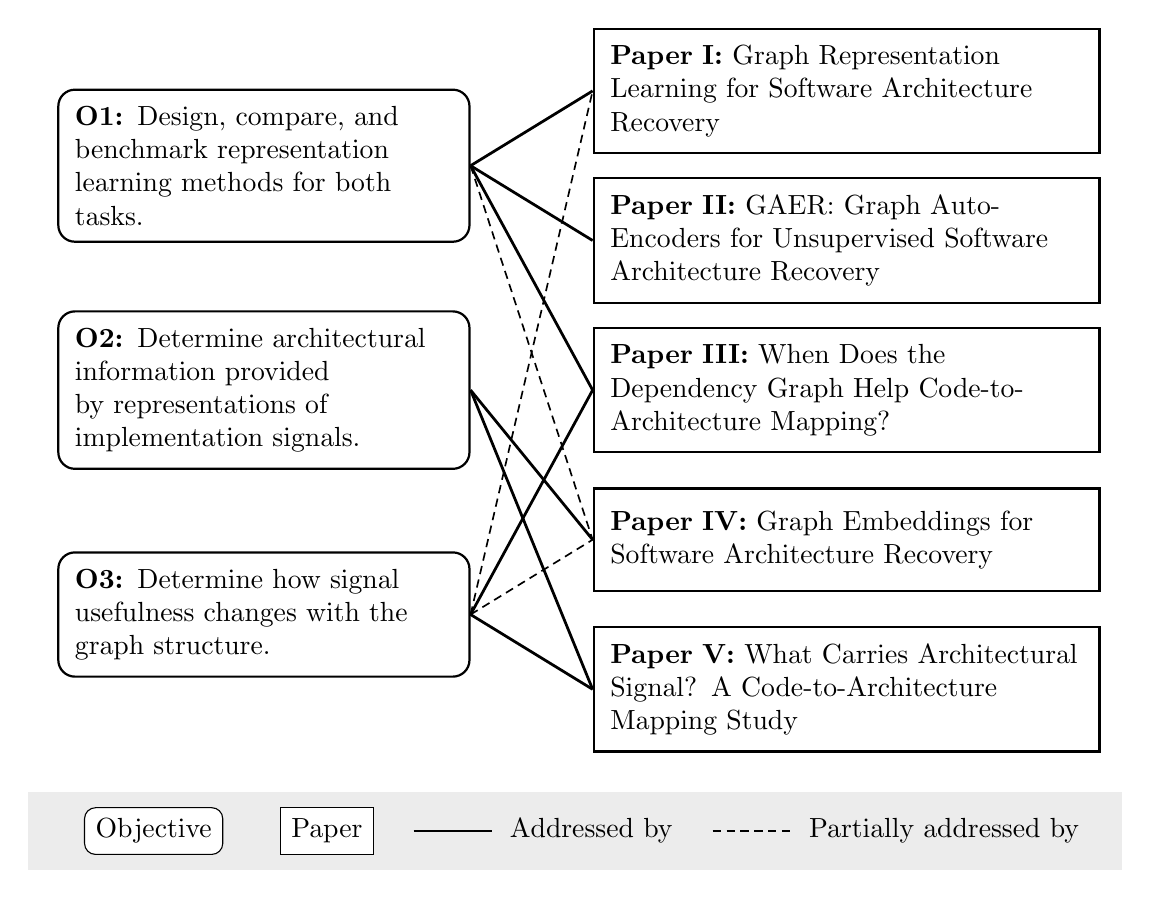
\begin{tikzpicture}[
    every node/.append style={execute at begin node={\sloppy\hyphenpenalty=10000\relax}},
    obj/.style={draw, rounded corners=6pt, line width=0.8pt, text width=4.8cm, align=left, inner sep=6pt, font=\figurefont\normalsize},
    pap/.style={draw, line width=0.8pt, text width=6cm, align=left, inner sep=6pt, minimum height=1.3cm, font=\figurefont\normalsize},
    full/.style={line width=1.0pt},
    part/.style={line width=0.6pt, dash pattern=on 3pt off 2pt}
]

% Papers
\node[pap] (P1) at (7.4, 0)     {\textbf{Paper I:} Graph Representation Learning for Software Architecture Recovery};
\node[pap] (P2) at (7.4,-1.90)  {\textbf{Paper II:} GAER: Graph Auto-Encoders for Unsupervised Software Architecture Recovery};
\node[pap] (P3) at (7.4,-3.80)   {\textbf{Paper III:} When Does the Dependency Graph Help Code-to-Architecture Mapping?};
\node[pap] (P4) at (7.4,-5.70)  {\textbf{Paper IV:} Graph Embeddings for Software Architecture Recovery};
\node[pap] (P5) at (7.4,-7.60)   {\textbf{Paper V:} What Carries Architectural Signal? A Code-to-Architecture Mapping Study};

% Objectives
\node[obj] (O1) at (0, -0.95) {\textbf{O1:} Design, compare, and benchmark representation learning methods for both tasks.};
\node[obj] (O2) at (0,-3.80)   {\textbf{O2:} Determine architectural information provided by representations of implementation signals.};
\node[obj] (O3) at (0,-6.65) {\textbf{O3:} Determine how signal usefulness changes with the graph structure.};

% Addressed by
\draw[full] (O1.east) -- (P1.west);
\draw[full] (O1.east) -- (P2.west);
\draw[full] (O1.east) -- (P3.west);
\draw[full] (O2.east) -- (P4.west);
\draw[full] (O2.east) -- (P5.west);
\draw[full] (O3.east) -- (P3.west);
\draw[full] (O3.east) -- (P5.west);

% Partially addressed by
\draw[part] (O1.east) -- (P4.west);
\draw[part] (O3.east) -- (P1.west);
\draw[part] (O3.east) -- (P4.west);

% Legend
\fill[gray!15] (-3.0,-8.9) rectangle (10.9,-9.9);
\node[draw, rounded corners=4pt, font=\figurefont\normalsize, inner sep=4pt, fill=white] at (-1.4,-9.4) {Objective};
\node[draw, font=\figurefont\normalsize, inner sep=4pt, fill=white] at (0.8,-9.4) {Paper};
\draw[full] (1.9,-9.4) -- (2.9,-9.4);
\node[font=\figurefont\normalsize, anchor=west] at (3.0,-9.4) {Addressed by};
\draw[part] (5.7,-9.4) -- (6.7,-9.4);
\node[font=\figurefont\normalsize, anchor=west] at (6.8,-9.4) {Partially addressed by};
\end{tikzpicture}